\subsection{Path Planning}
The entire 3 dimensional environment is divided into N unit volume cubes, centred at integer coordinates.
 
A modified A* algorithm is used as the basis for path planning. It is augmented by the depth map discussed in the previous section. The interfacing between the algorithm and the generated depth map will be discussed in the subsequent section.

The following implicit data structures and objects are maintained by the agent controller object:
 
\textbf{set\_visited}
A set of previously visited nodes
 
\textbf{set\_prospects}
The currently available prospects for immediate motion
 
\textbf{stack\_active}
A stack of nodes on the currently active path
 
\textbf{to\_cube}
The highest priority cube in the immediate surroundings on the path to destination

Two types of step movement policies were examined for this control policy:
\begin{enumerate}
\item 4-connected policy
\item 8-connected policy
\end{enumerate}

Two distance heuristics were compared in the experiment:
\begin{enumerate}
\item Manhattan distance
\item Euclidean distance
\end{enumerate}

\subsection{Interfacing depth map with path planner}

The entire 3 dimensional environment is divided into virtual unit volume cubes, centred at integer coordinates. There are 8 immediately neighbouring cubes to which the agent can move. The path planner locally generates the next cube towards which it intends to move based on the heuristic.

The agent receives two 200x200 input image streams from the left and right cameras based on which it must plan it's short term path and avoid obstacles. The agent step rotates and faces the heuristic selection. The agent uses the trained CNN to generate a single 200x200 pixel depth map from the stereo image camera stream.

This depth map is filtered and cropped to focus on the target window W for the agent, and mean intensity statistics are computed. If the agent evaluates the mean intensity to be above a threshold T, it decides that the heuristic generated next-cube isn't safe for traversal and directs it to present an alternate option. This process continues until the heuristic selects a subsequent neighbouring cube with no detected obstacles.

\begin{algorithm}
\caption{Experiment Workflow}
\label{alg1}
\begin{algorithmic}[1]
\STATE Import Blender model, and obstacles from the Shapenet Database
\STATE Initialize neural network and load CNN model weights
\STATE Two cubes are selected (src\_cube or dest\_cube)
\STATE Ensure there is no collision with src\_cube or dest\_cube
\STATE Initialize agent controller with these initial values
\STATE Interface agent controller with left and right camera stream
\STATE Start game and log the step counts
\STATE End log when destination reached
\end{algorithmic}
\end{algorithm}

\begin{figure}
  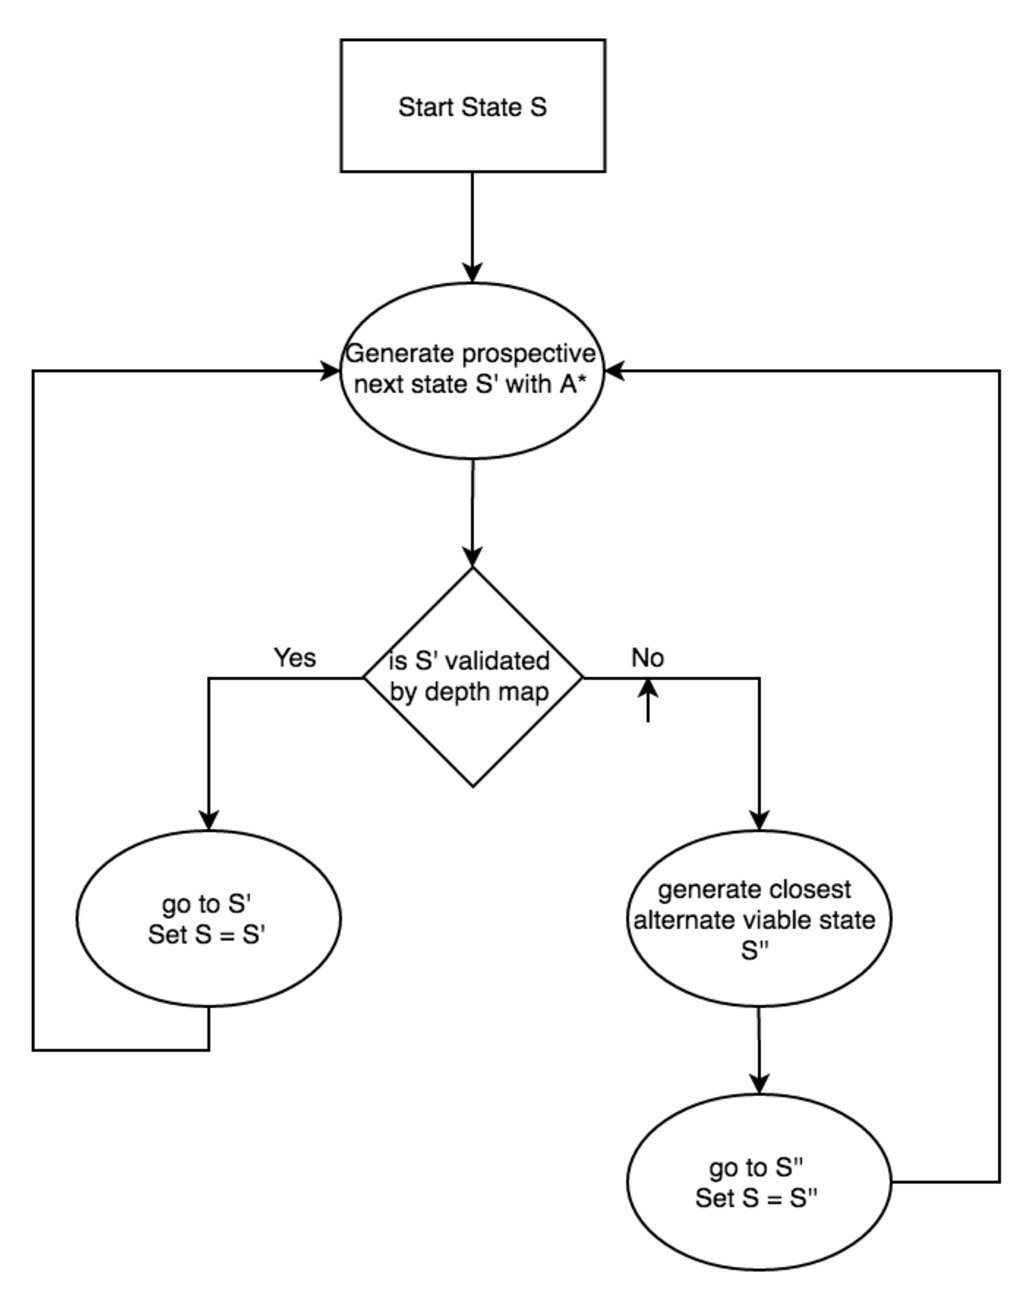
\includegraphics[width=\linewidth]{images/flowchart.png}
  \caption{Interfacing depth map with path planner}
  \label{fig:flowchart1}
\end{figure}